\documentclass[12pt]{article}

\usepackage{geometry}
 \geometry{
 a4paper,
 total={170mm,257mm},
 left=20mm,
 top=20mm,
 }
\usepackage{polyglossia}
\setmainlanguage{russian} 
\setotherlanguage{english}
\setmainfont{FreeSerif}
\setsansfont{FreeSans}
\setmonofont{FreeMono}

\usepackage{sectsty}

\sectionfont{\fontsize{14}{15}\selectfont}

\usepackage{graphicx} 
\graphicspath{{images/}}
\usepackage{subcaption}

\title{Задача № 8 \\ 
Нахождение наименьшего покрытия простого графа}
\author{Гига Максим М8О-113Б-23}
\date{2024}
\begin{document}
\maketitle

\section{Теоретические сведения. Описание алгоритма}

Простым графом называют такой граф $G = (X \cup Y, \Gamma)$, что
\begin{enumerate}
    \item $X \cap Y = \emptyset$
    \item $(\forall X_i \in X) \Gamma X_i \subset Y$
          или $\Gamma^{-1} X_i = \emptyset$
    \item $(\forall Y_j \in Y) \Gamma Y_j = \emptyset$
\end{enumerate}

Простой граф будем обозначать $G = (X, Y, \Gamma)$

Простой граф можно определить также как многозначное
отображение $\Gamma$ конечного множества $X$ в конечное
множество $Y$

Покрытием простого графа $G = (X, Y, \Gamma) = (X, Y, U)$ называют
такое подмножество дуг $W \subset U$, что любая вершина графа
инцидентна по крайней мере одной дуге из $W$

Для того, чтобы простой граф обладал покрытием необходимо и достаточно
выполнение условий:
\begin{enumerate}
    \item $(\forall X_i \in X) \Gamma X_i \ne \emptyset$
    \item $(\forall Y_j \in Y) \Gamma^{-1} Y_j \ne \emptyset$
\end{enumerate}

Минимальное покрытие $W_0$ – это покрытие с минимальным $|W_0|$
то есть с наименьшим числом дуг.

\section{Описание алгоритма, использующего булево
  матричное представление}

Опишем алгоритм позволяющий получить минимальное покрытие
простого графа \\ $G = (X, Y, \Gamma)$, представленного
в виде булевой матрицы $||M||$ размера $m \times n$

\begin{enumerate}
    \item Сопоставим каждой строке $X_i$ матрицы $||M||$
          число $F_i$, равное сумме ее элементов,
          и каждому столоцу $Y_j$ – число $G_j$, равное сумме
          его элементов
    \item Если $\sum F_i = \sum G_j = max(m, n)$ то
          множество дуг, соответствующих единицам,
          дает минимальное покрытие. Если
          $\sum F_i = \sum G_j > max(m, n)$
          то заменяем последовательно
          в произвольном порядке $0$ каждую из единиц
          (условливаясь при этом писать $\widehat{1}$ вместо $0$),
          для которой $F_i > 1$ и $G_j > 1$.
    \item В каждой строке с $F_i > 1$ ищем такую
          $1$, что её столбце найдется
          такая $\widehat{1}$, что в строке,
          содержащей эту $\widehat{1}$, есть неотмеченная $1$
          с $G_j > 1$. Если $G_j > 1$, то найденная $\widehat{1}$
          заменяется на $1$, а найденные $1$ заменяются на
          $\widehat{1}$. $F_i$ и $G_j$ обновляются.
          Если, действуя по этому алгоритму,
          невозможно увеличить число $\widehat{1}$,
          то $1$ дают минимальное покрытие.
\end{enumerate}

\section{Логическая блок-схема алгоритма}

\section{Оценка сложности алгоритма}

Наибольшую сложность имеет подпрограмма, исполняющая
пункт 3 алгоритма. Пункт 1 имеет сложность $O(n * m)$
Пункт 2 имеет сложность $O(n * m)$
Пункт 3 имеет сложность $O(n^2 * m^2)$, что соответсвует $4$
вложенным циклам, два из которыз проходят по строкам ($n$) и
два по столбцам ($m$).

\section{Тестовые примеры}

\section{Скриншоты программы}

\begin{figure}[h]
    \centering
    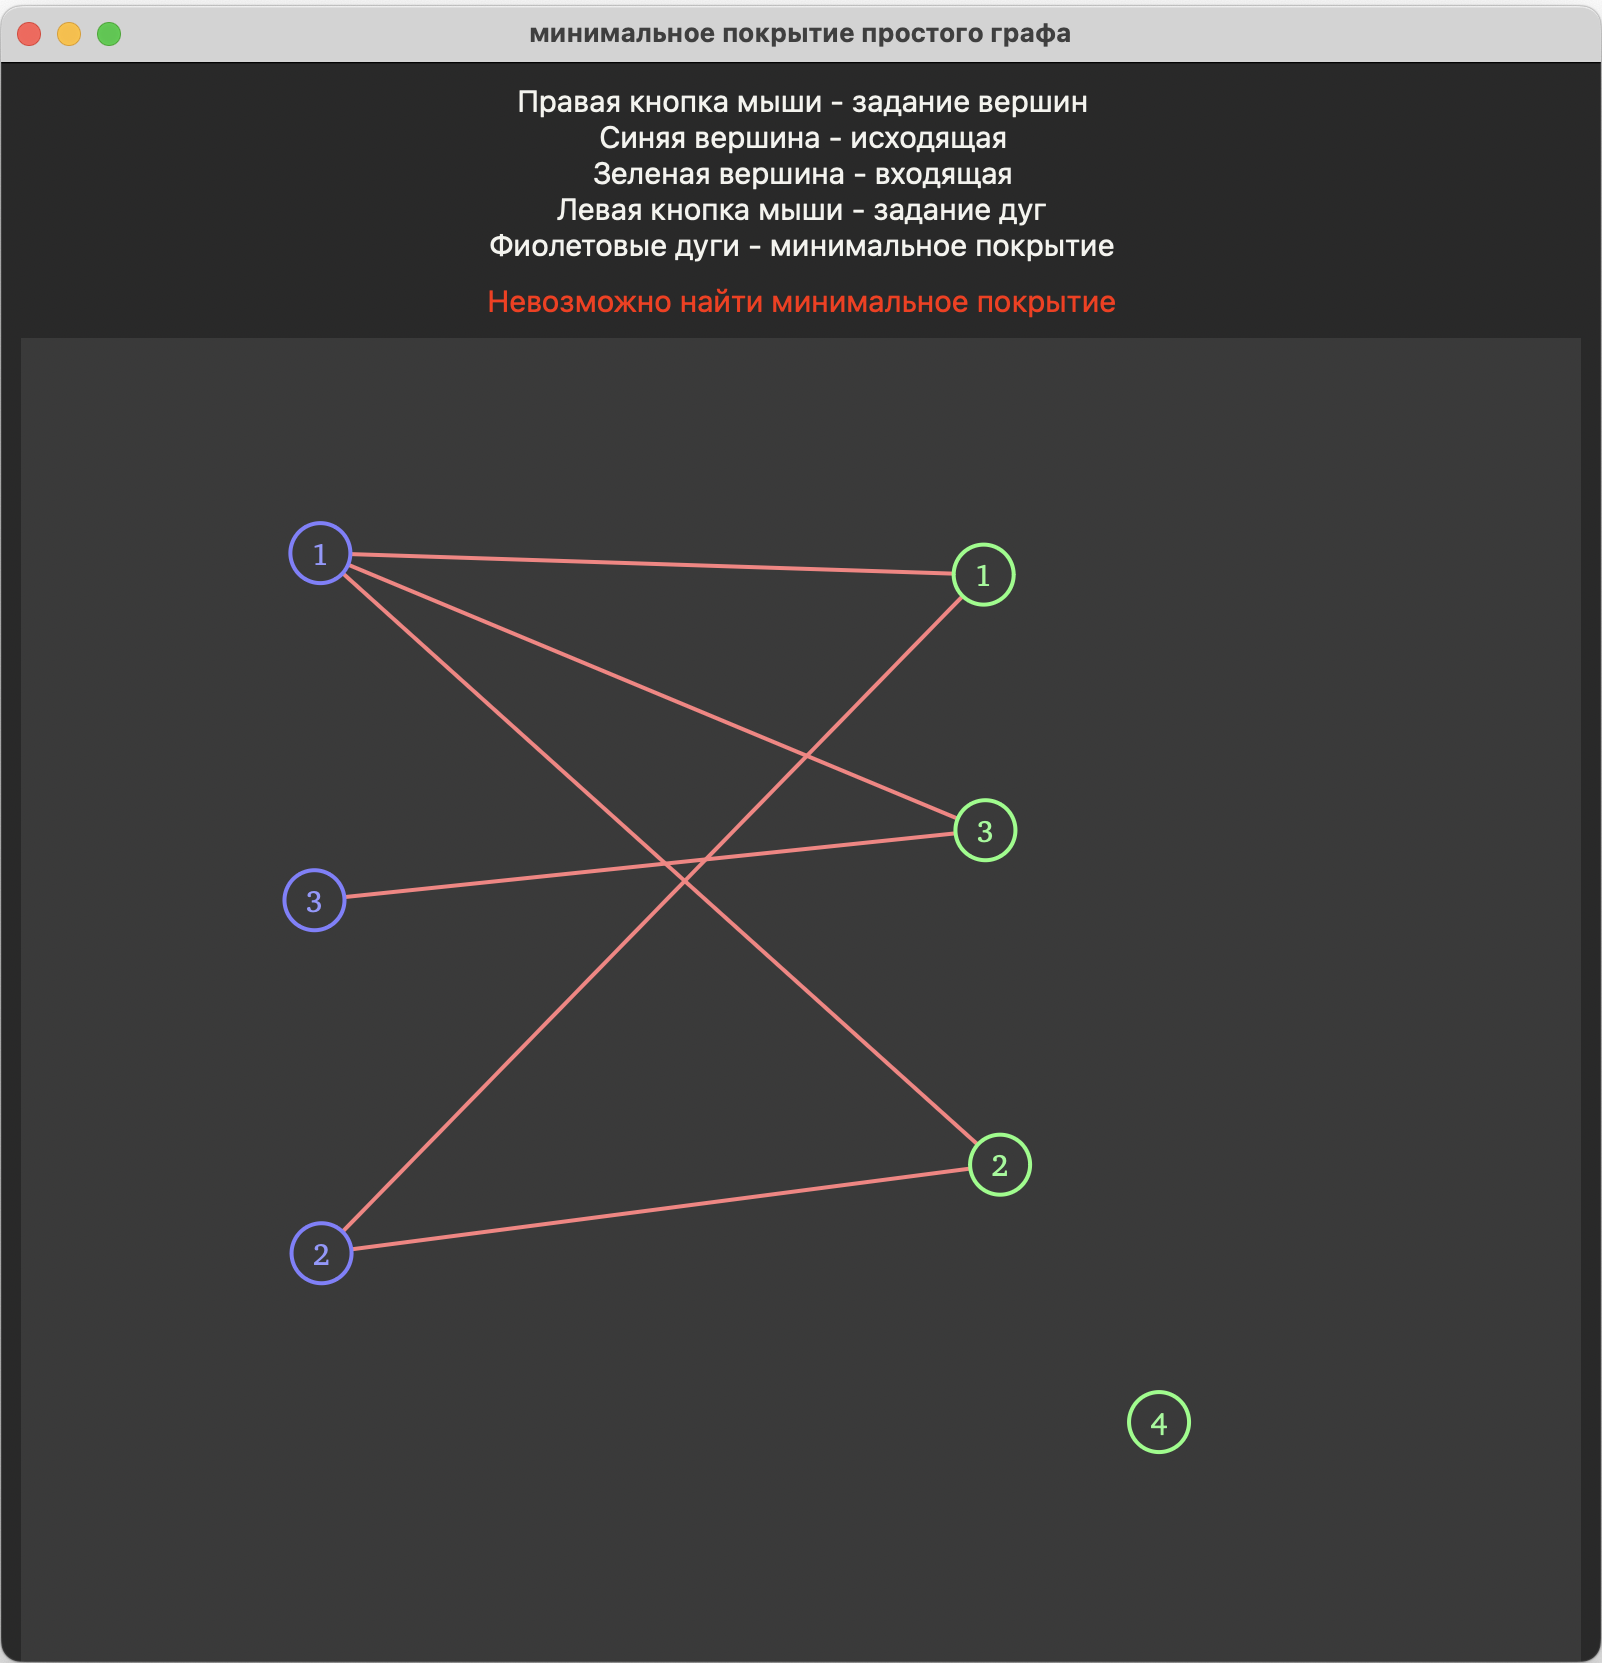
\includegraphics[width=0.5\textwidth]{screenshot1.png}
    \caption{Выдача ошибки при невозможности
        нахожения минимального покрытия}
    \label{fig:failure_example}
\end{figure}

\begin{figure}[h]
    \begin{subfigure}{0.3\textwidth}
        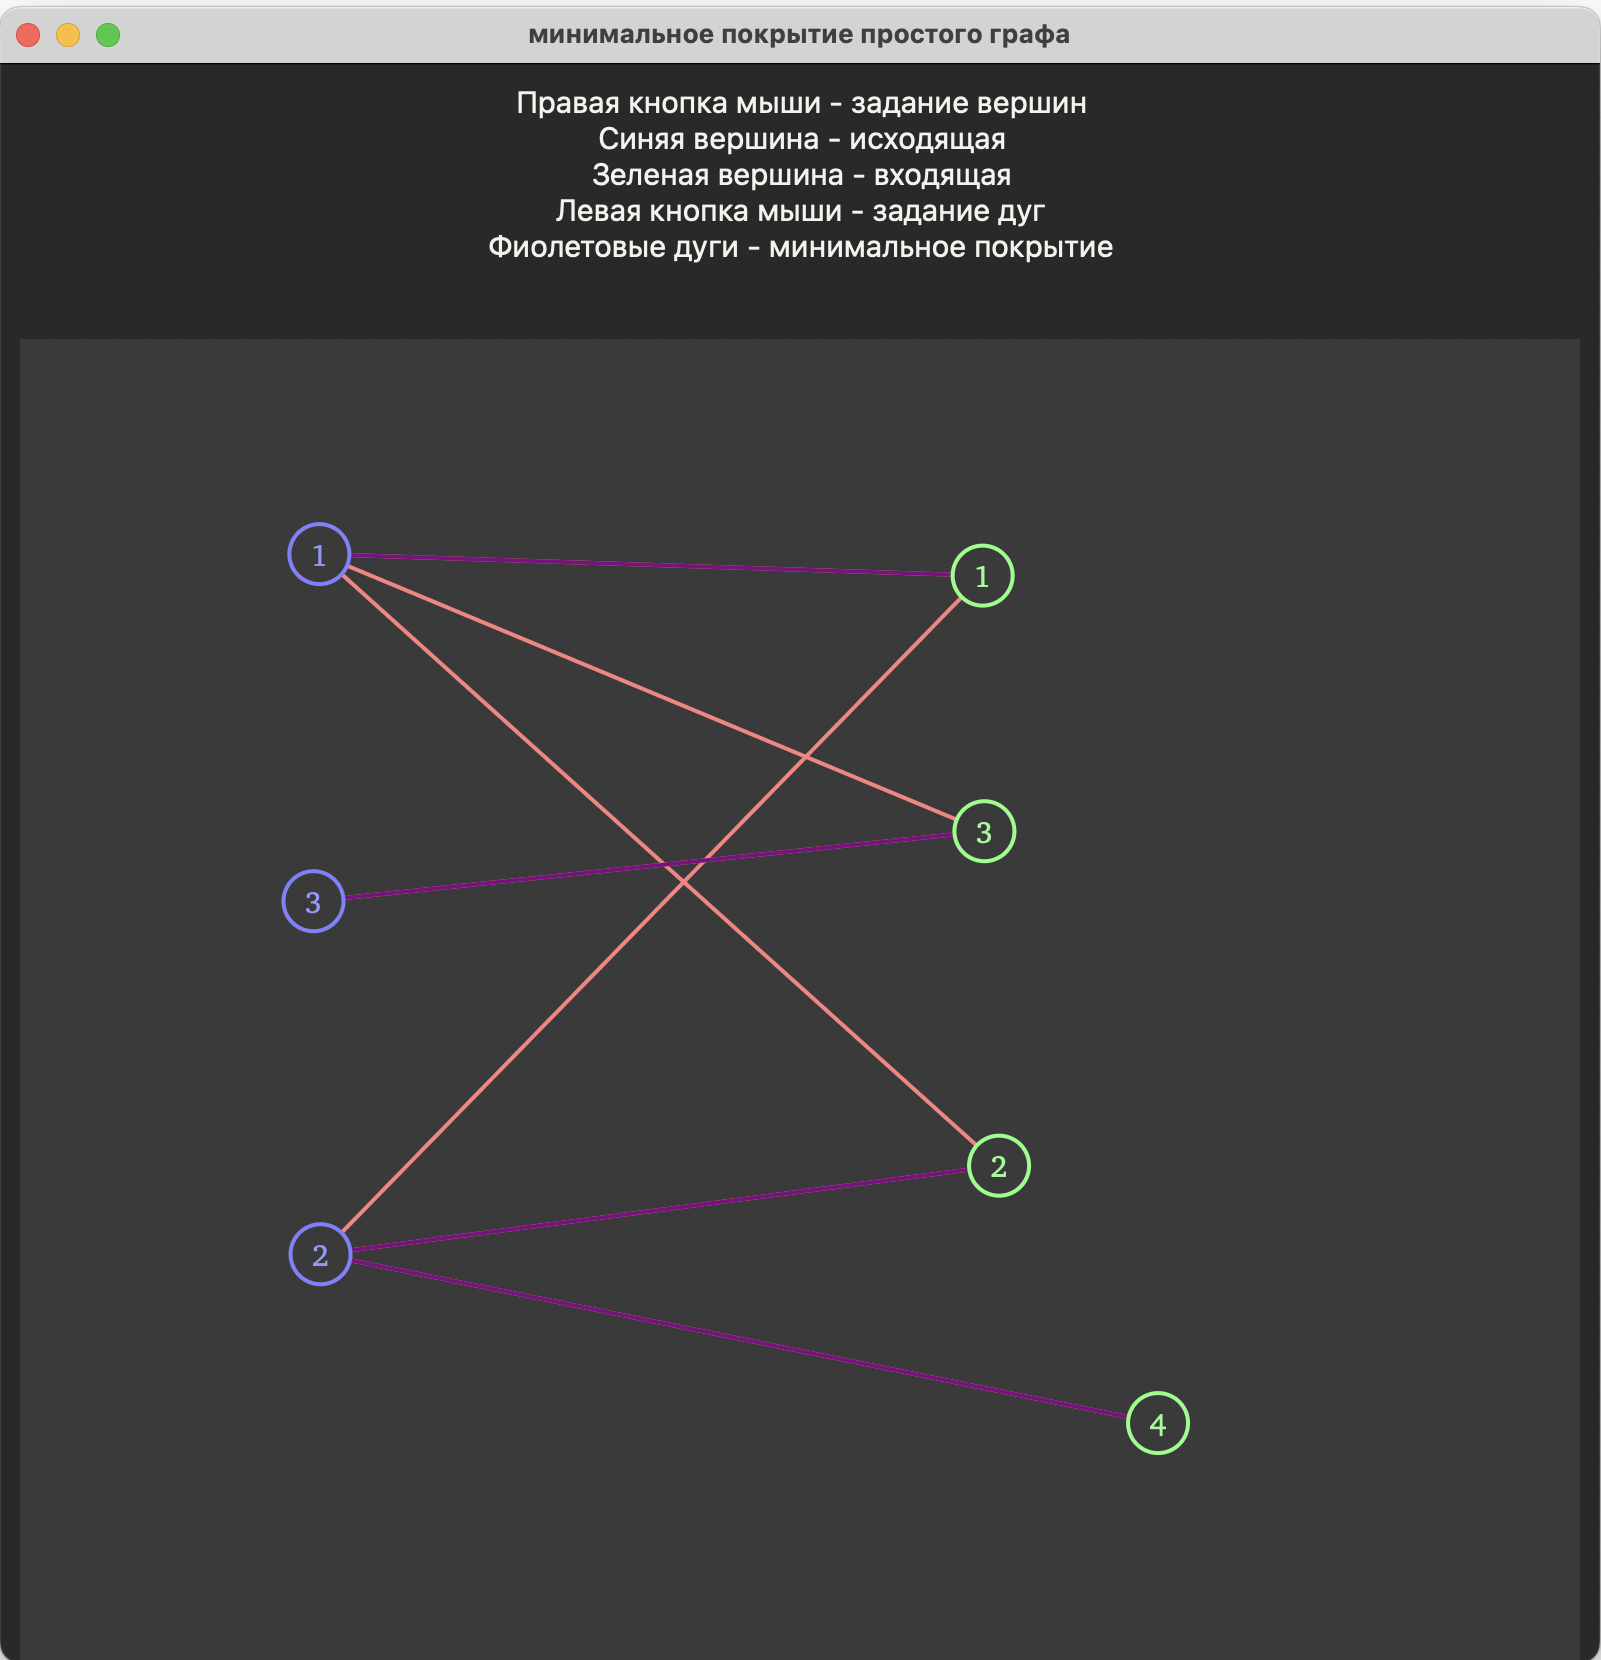
\includegraphics[width=1\textwidth]{screenshot2.png}
        \caption{Пример 1}
        \label{fig:subim1}
    \end{subfigure}
    \begin{subfigure}{0.3\textwidth}
        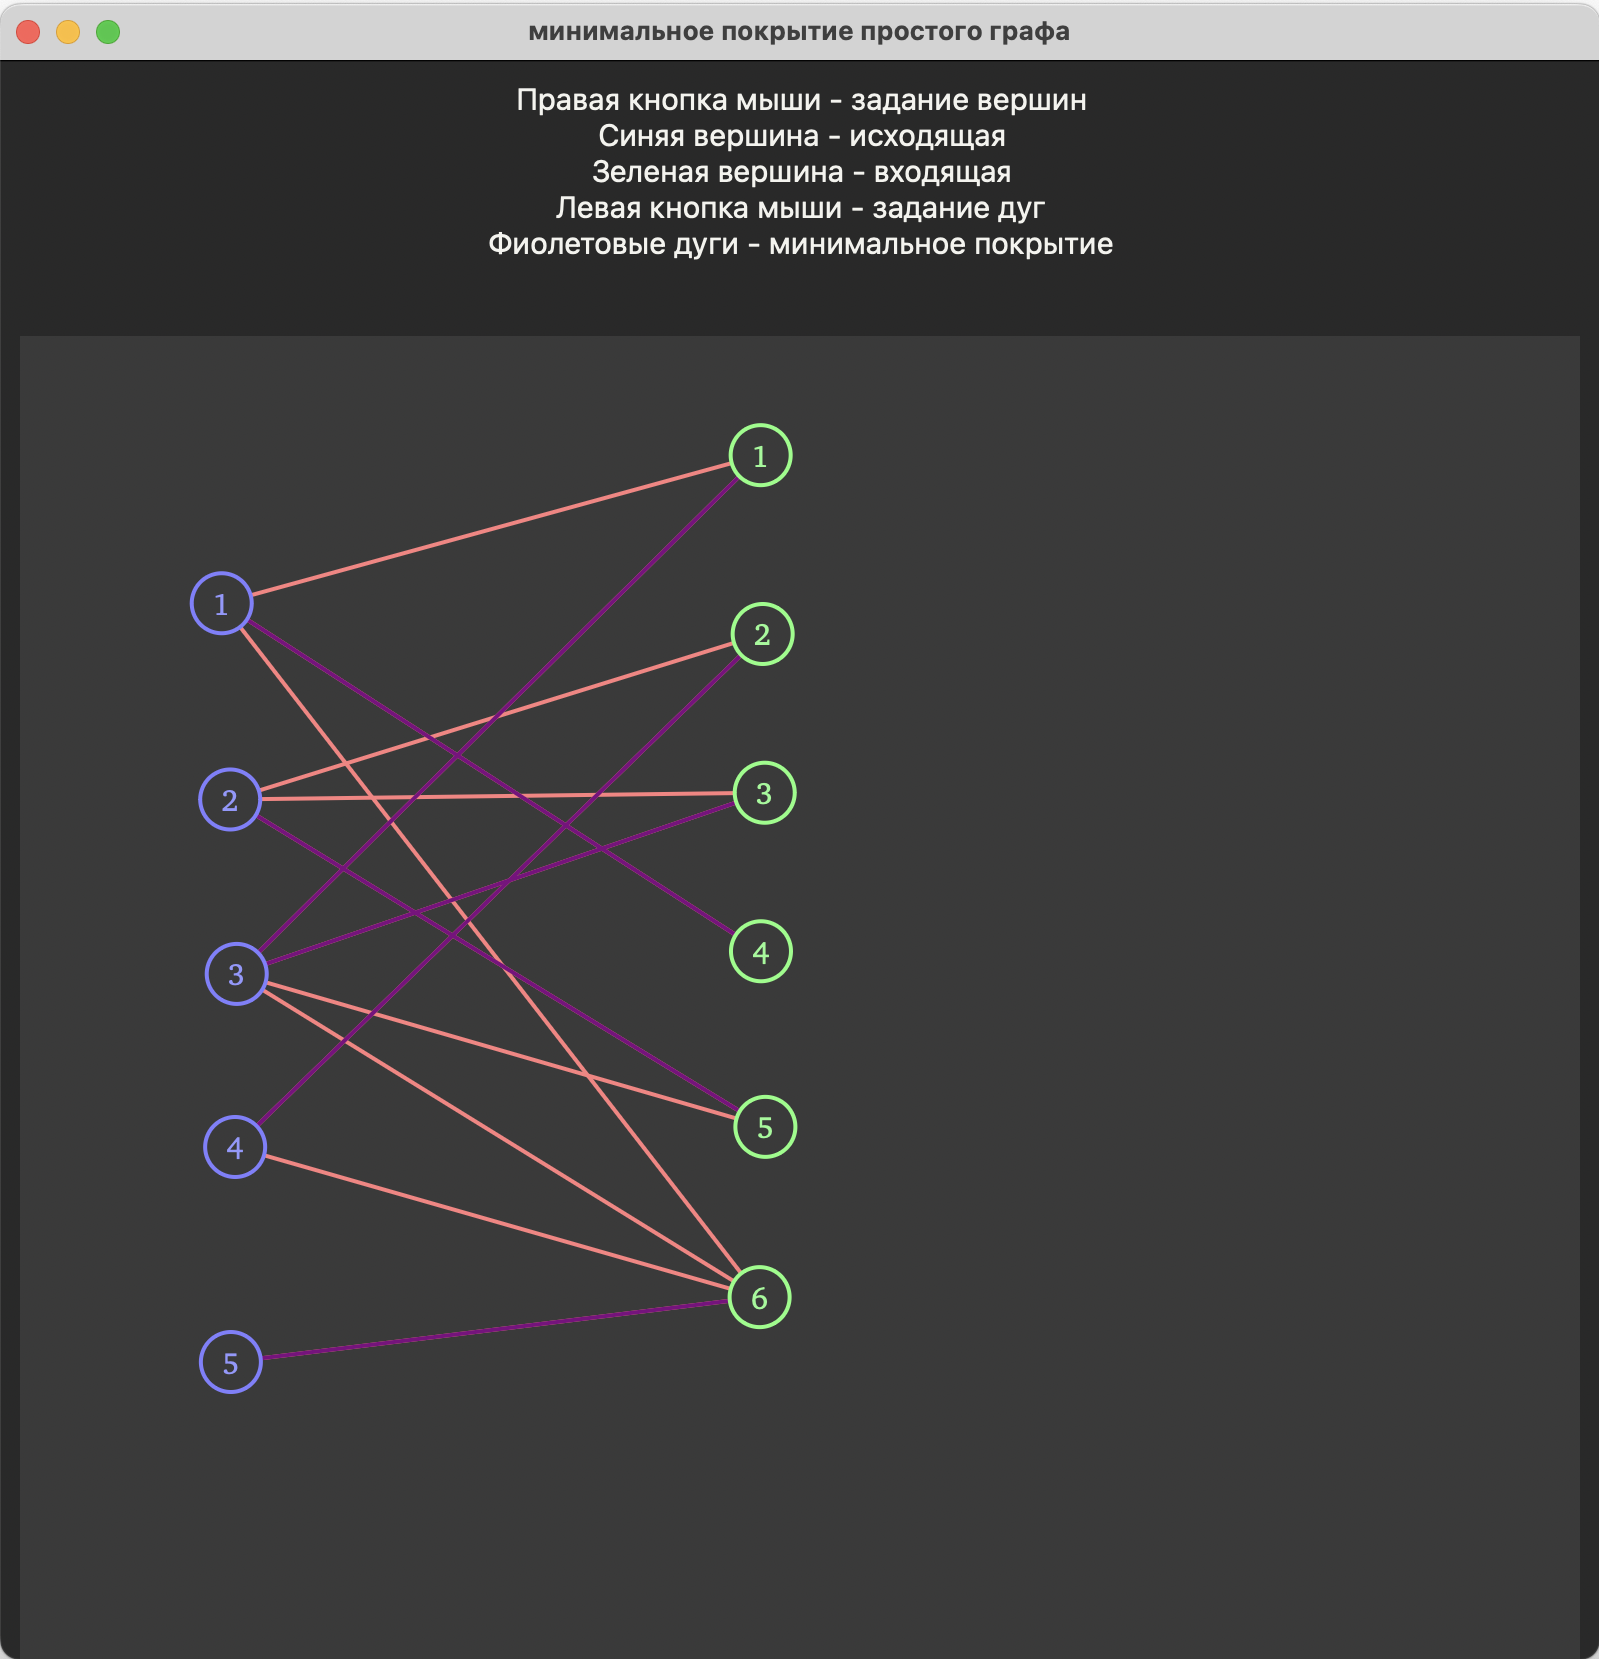
\includegraphics[width=1\textwidth]{screenshot3.png}
        \caption{Пример 2}
        \label{fig:screenshot3}
    \end{subfigure}
    \begin{subfigure}{0.3\textwidth}
        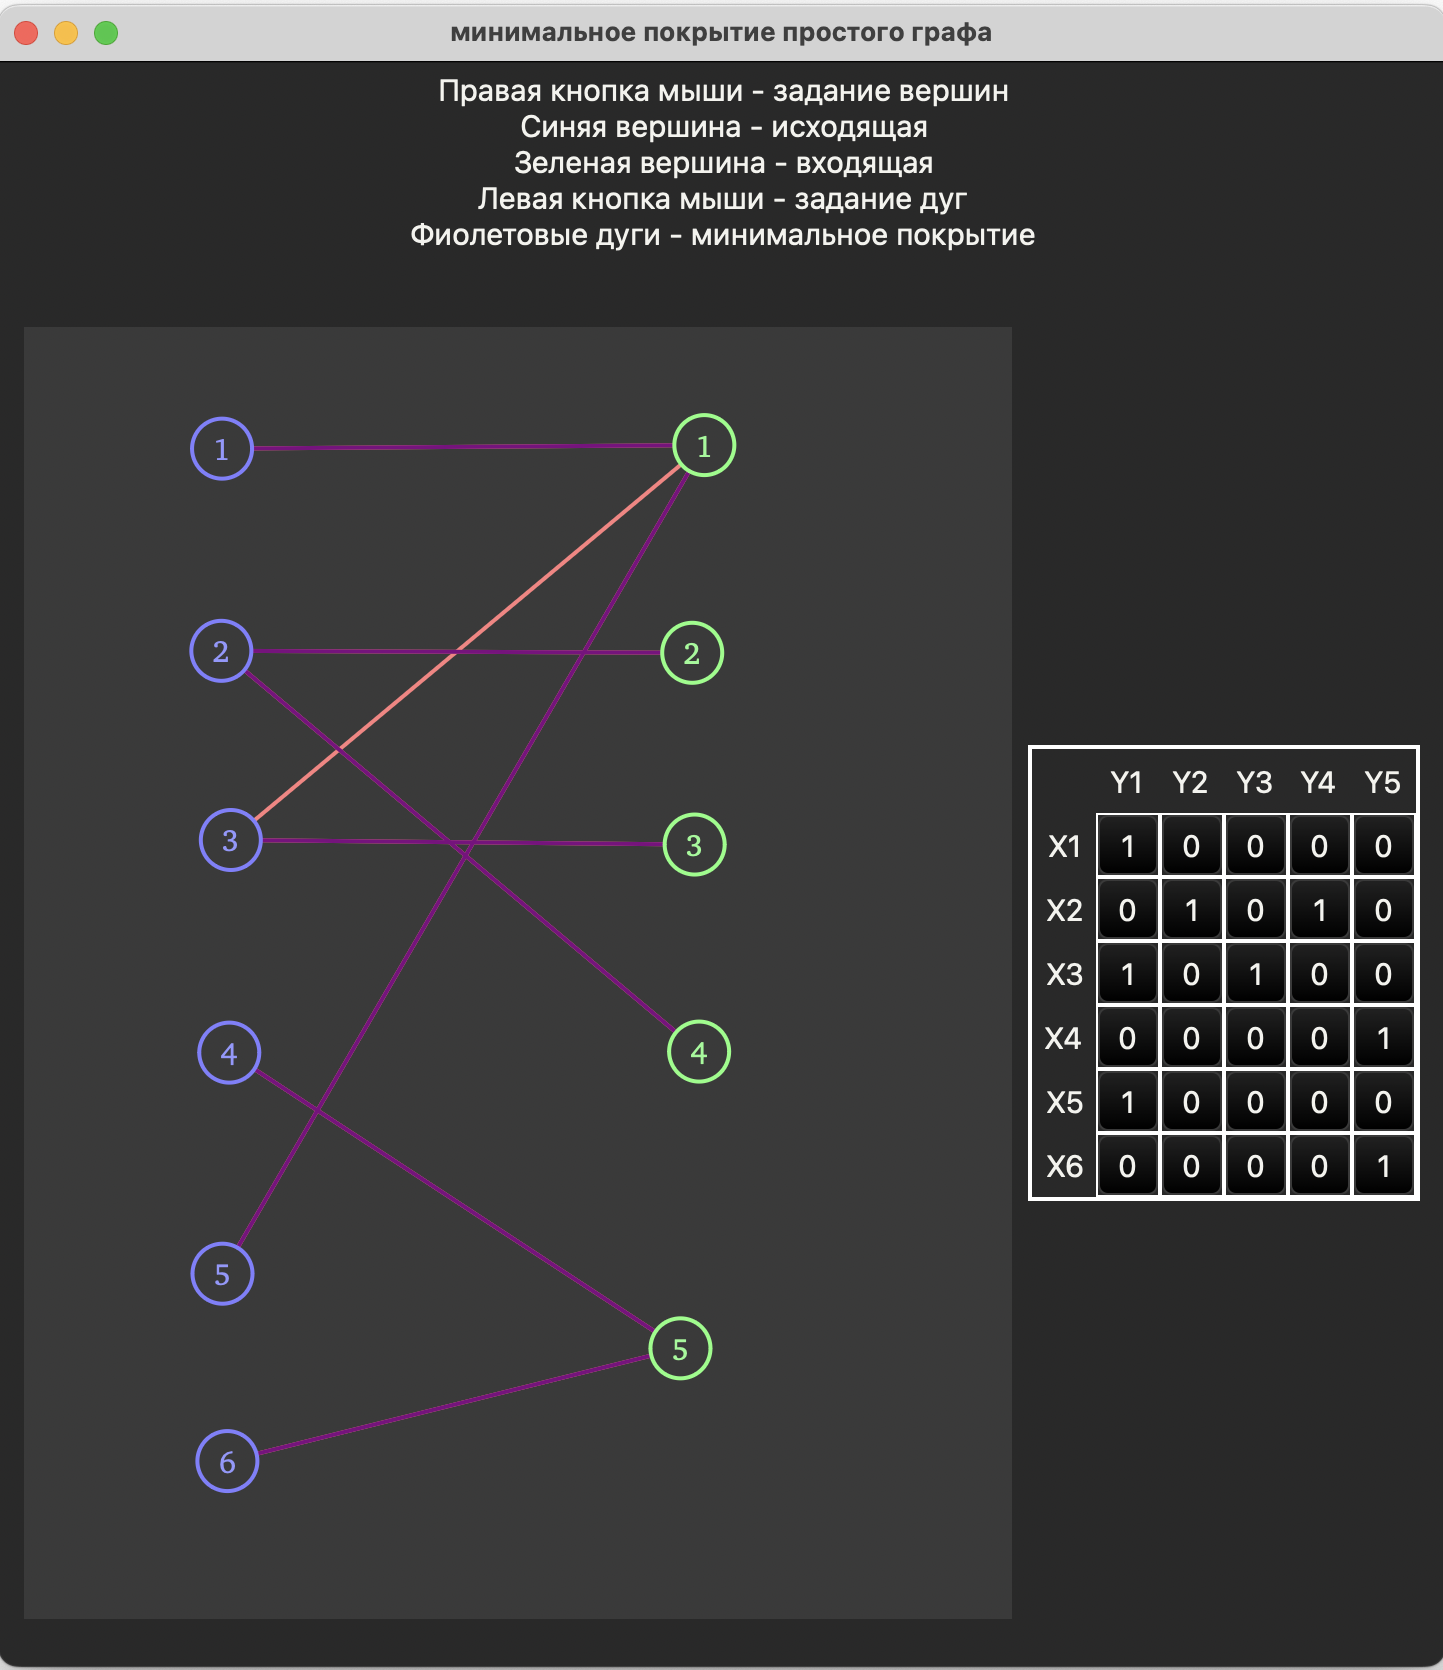
\includegraphics[width=1\textwidth]{screenshot4.png}
        \caption{Пример 3}
        \label{fig:screenshot4}
    \end{subfigure}
    \caption{Успешное нахождение минимального покрытия}
    \label{fig:success_example}
\end{figure}


\section{Пример прикладной задачи}

\end{document}